%!TEX TS-program = XeLaTeX
%!TEX TS-program = XeLaTeX
\documentclass[11pt]{article}

\usepackage{amssymb}
\usepackage{amsthm}
\usepackage{amsmath}
\usepackage{mathtools}

\usepackage{fancyhdr}
\usepackage{graphicx}
\usepackage[top=3cm, left=2cm, right=2cm, headheight = 90pt]{geometry}
\usepackage{xltxtra}
\usepackage[font=small,labelfont=bf]{caption}

\usepackage{multicol}

\renewcommand{\theenumi}{\alph{enumi}}


\def\leq{\leqslant}
\def\geq{\geqslant}
\def\N{\mathbb N}
\def\R{\mathbb R}
\def\Z{\mathbb Z}
\DeclarePairedDelimiter\set\{\}

\def\prob{}

\theoremstyle{definition}
\newtheorem{problem}{\prob}


\pagestyle{fancy}

%%!TEX TS-program = XeLaTeX

\fancyfoot[CE,CO]{}  % this is to remove page numbers (as you might want for single page docs)

%%!TEX TS-program = XeLaTeX
\renewcommand{\figurename}{Attēls}

\fancyhead[C]{{\Large\bf Games and Processes - Solutions}\\ \date}

\renewcommand{\theenumi}{\alph{enumi}}


\begin{document}

\noindent
 
\filbreak

%1
\begin{problem}
\textit{[IMO2009SLC1]}


\textbf{Problem}

Consider $2009$ cards, each having one gold side and one black side, lying in a line on a long table. Initially all cards show their gold sides. Two players, standing by the same long side of the table, play a game with alternating moves. Each move consists of choosing a block of $50$ consecutive cards, the leftmost of which is showing gold, and turning them all over, so those with showed gold now show black and vice versa. The last player who can make a legal move wins.
\begin{enumerate}
\item Does the game necessarily end?
\item Does there exist a winning strategy for the starting player?
\end{enumerate}


\textbf{Solution - binary representation; strong variant; coloring a subset; analysing whole ws inductuion}
\begin{enumerate}
\item If we denote gold cards by $1$, and black by $0$, the entire sequence of cards  corresponds to a number in binary representation. After each of the moves, the number decreases, hence the game has to end.
\item We will show that second player wins a game no matter how the players play. Consider the cards whose position (counted from the right) is divisible by $50$. There is a total of $40$ such cards, and in each move exactly one of this cards is turned over. In the beginning, all $40$ of these cards are $1$, and in the end all $40$ are $0$, hence the second player must win.
\end{enumerate}
\end{problem}
%

\filbreak
%2
\begin{problem}
\textit{[IMO2015SLC1]}

\textbf{Problem}

 In Lineland there are $n \ge 1$ towns, arranged along a road running from left to right. Each town has a left bulldozer (put to the left of the town and facing left) and a right bulldozer (put to the right of the town and facing right). The sizes of the $2n$ bulldozers are distinct. Every time when a right and a left bulldozer confront each other, the larger bulldozer pushes the smaller one off the road. On the other hand, the bulldozers are quite unprotected at their rears; so, if a bulldozer reaches the rear-end of another one, the first one pushes the second one off the road, regardless of their sizes. 
 
Let $A$ and $B$ be two towns, with $B$ being to the right of $A$. We say that town $A$ can \textit{sweep town B away} if the right bulldozer of $A$ can move over to $B$ pushing off all bulldozers it meets. Similarly, $B$ can sweep $A$ away if the left bulldozer of $B$ can move to $A$ pushing off all bulldozers of all towns on its way. 

Prove that there is exactly one town which cannot be swept away by any other one. 


\textbf{Solution - Induction}

 Let $T_1,T_2,\dots,T_n$ be the towns enumerated from left to right. Observe first that, if town $T_i$ can sweep away town $T_j$, then $T_i$ also can sweep away every town located between $T_i$ and $T_j$. 
 
 We prove the problem statement by strong induction on n. The base case $n = 1$ is trivial. 
 
 For the induction step, we first observe that the left bulldozer in $T_1$ and the right bulldozer in $T_n$ are completely useless, so we may forget them forever. Among the other $2n-2$ bulldozers, we choose the largest one. Without loss of generality, it is the right bulldozer of some town $T_k$ with $k < n$. Surely, with this large bulldozer $T_k$ can sweep away all the towns to the right of it. Moreover, none of these towns can sweep $T_k$ away; so they also cannot sweep away any town to the left of $T_k$. Thus, if we remove the towns $T_k+1,T_k+2,\dots,T_n$, none of the remaining towns would change its status of being (un)sweepable away by the others. 
 
 Applying the induction hypothesis to the remaining towns, we find a unique town among $T_1,T_2,\dots,T_k$ which cannot be swept away. By the above reasons, it is also the unique such town in the initial situation. Thus the induction step is established.

\end{problem}
\filbreak
%3
\begin{problem}
\textit{[IMO2015SLC1]}

\textbf{Problem}

Several positive integers are written in a row. Iteratively, Alice chooses two adjacent numbers $x$ and $y$ such that $x > y$ and $x$ is to the left of $y$, and replaces the pair $(x,y)$ by either $(y + 1,x)$ or $(x − 1,x)$. 

Prove that she can perform only finitely many such iterations.

\textbf{Solution - bounded variant; digit representation }

Firstly observe that maximum element $M$ of this sequence  does not change during allowed operations.

Now, consider a \textit{characteristic} $C$ of particular sequence $v$ of integers in our problem. Value of $C$ would be calculated by inverting string $v$ and then interpreting elements of this invcerted sequence as digits in $M$-base counting system.

I.e. if original $v$ consists of $k$ elements $v_1, v_2, \dots, v_k$ then $C = v_k \times M^{k-1} + v_{k-1} \times M^{k-2} + v_{k-2}\times M^{k-3} + \dots + v_2 \times M^{1} + v_1 \times M^{0}$

It is easy to see that every allowed operation strictly increases $C$, but on other hand $C$ is upper bound by $M^k-1$, so the process must stop at some point.
\end{problem}
\filbreak
%4
\begin{problem}
$[IMO2011SLC3]$

\textbf{Problem}

Let $S$ be a finite set of at least two points in the plane. Assume that no three points of $S$ are collinear. By a windmill we mean a process as follows. Start with a line $l$ going through a point $P \in S$. Rotate $l$ clockwise around the pivot $P$ until the line contains another point $Q$ of $S$. The point $Q$ now takes over as the new pivot. This process continues indefinitely, with the pivot always being a point from $S$. Show that for a suitable $P \in S$ and a suitable starting line $l$ containing $P$, the resulting windmill will visit each point of $S$ as a pivot infinitely often.

\textbf{Solution - continuous process, geometry, invariant}

Give the rotating line an orientation and distinguish its sides as the \textit{oranje} side and the \textit{blue} side. Notice that whenever the pivot changes from some point $T$ to another point $U$, after the change, $T$ is on the same side as $U$ was before. Therefore, the number of elements of $S$ on the oranje side and the number of those on the blue side remain the same throughout the whole process (except for those moments when the line contains two points).

\begin{center}
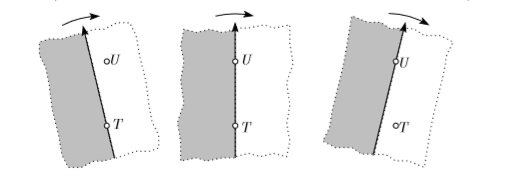
\includegraphics[width=18cm]{windmill.png}
\captionof{figure}{Number of points staying constant on each side of the windmill}
\label{fig:windmill}
\end{center}

First consider the case that $|S| = 2n + 1$ is odd. We claim that through any point $T \in S$, there is a line that has n points on each side. To see this, choose an oriented line through $T$ containing no other point of $S$ and suppose that it has $n + r$ points on its oranje side. If $r = 0$ then we have established the claim, so we may assume that $r \ne 0$. As the line rotates through $180\degree$ around $T$, the number of points of $S$ on its oranje side changes by $1$ whenever the line passes through a point; after $180\degree$, the number of points on the oranje side is $n−r$. Therefore there is an intermediate stage at which the oranje side, and thus also the blue side, contains $n$ points.

 Now select the point $P$ arbitrarily, and choose a line through $P$ that has $n$ points of $S$ on each side to be the initial state of the windmill. 
We will show that during a rotation over $180\degree$, the line of the windmill visits each point of $S$ as a pivot. To see this, select any point $T$ of $S$ and select a line $l$ through $T$ that separates $S$ into equal halves. The point $T$ is the unique point of $S$ through which a line in this direction can separate the points of $S$ into equal halves (parallel translation would disturb the balance). Therefore, when the windmill line is parallel to $l$, it must be $l$ itself, and so pass through $T$.

Next suppose that $|S| = 2n$. Similarly to the odd case, for every $T \in S$ there is an oriented line through $T$ with $n−1$ points on its oranje side and n points on its blue side. Select such an oriented line through an arbitrary $P$ to be the initial state of the windmill. 

We will now show that during a rotation over $360\degree$, the line of the windmill visits each point of $S$ as a pivot. To see this, select any point $T$ of $S$ and an oriented line $l$ through $T$ that separates $S$ into two subsets with $n − 1$ points on its oranje and n points on its blue side. Again, parallel translation would change the numbers of points on the two sides, so when the windmill line is parallel to $l$ with the same orientation, the windmill line must pass through $T$.

\textbf{Comment} One may shorten this solution in the following way. 

Suppose that $|S| = 2n + 1$. Consider any line $l$ that separates $S$ into equal halves; this line is unique given its direction and contains some point $T \in S$. Consider the windmill starting from this line. When the line has made a rotation of $180\degree$, it returns to the same location but the oranje side becomes blue and vice versa. So, for each point there should have been a moment when it appeared as pivot, as this is the only way for a point to pass from on side to the other. 

Now suppose that $|S| = 2n$. Consider a line having $n−1$ and $n$ points on the two sides; it contains some point $T$. Consider the windmill starting from this line. After having made a rotation of $180\degree$, the windmill line contains some different point $R$, and each point different from $T$ and $R$ has changed the color of its side. So, the windmill should have passed through all the points.


\end{problem}

%5
\begin{problem}
$[IMO2009SLC5]$

\textbf{Problem}

Five identical empty buckets of 2-liter capacity stand at the vertices of a regular pentagon. Cinderella and her wicked Stepmother go through a sequence of rounds: At the beginning of every round, the Stepmother takes one liter of water from the nearby river and distributes it arbitrarily over the five buckets. Then Cinderella chooses a pair of neighboring buckets, empties them into the river, and puts them back. Then the next round begins. The Stepmother’s goal is to make one of these buckets overflow. Cinderella’s goal is to prevent this. 

Can the wicked Stepmother enforce a bucket overflow?

*What should be the volume of buckets for answer to change?


\textbf{Solution - complex invariant }

 No, the Stepmother cannot enforce a bucket overflow and Cinderella can keep playing forever. Throughout we denote the five buckets by $B_0,B_1,B_2,B_3$, and $B_4$, where $B_k$ is adjacent to bucket $B_{k−1}$ and $B_{k+1}$ $(k = 0,1,2,3,4)$ and all indices are taken modulo $5$. Cinderella enforces that the following three conditions are satisfied at the beginning of every round: 
 \begin{enumerate}
 \item Two adjacent buckets (say $B_1$ and $B_2$) are empty. 
 \item The two buckets standing next to these adjacent buckets (here $B_0$ and $B_3$) have total contents at most $1$. 
 \item The remaining bucket (here $B_4$) has contents at most $1$. 
\end{enumerate} 
 These conditions clearly hold at the beginning of the first round, when all buckets are empty. 
 
 Assume that Cinderella manages to maintain them until the beginning of the $r$-th round $(r \ge 1)$. Denote by $x_k (k = 0,1,2,3,4)$ the contents of bucket $B_k$ at the beginning of this round and by $y_k$ the corresponding contents after the Stepmother has distributed her liter of water in this round. 
 
 By the conditions, we can assume $x_1 = x_2 = 0, x_0 + x_3 \le 1$ and $x_4 \le 1$. Then, since the Stepmother adds one liter, we conclude $y_0+y_1+y_2+y_3 \le 2$. This inequality implies $y_0+y_2 \le 1$ or $y_1 + y_3 \le 1$. For reasons of symmetry, we only consider the second case. 
 
 Then Cinderella empties buckets $B_0$ and $B_4$. At the beginning of the next round $B_0$ and $B_4$ are empty (condition (a) is fulfilled), due to $y_1+y_3 \le 1$ condition (b) is fulfilled and finally since $x_2 = 0$ we also must have $y_2 \le 1$ (condition (c) is fulfilled). 
 
 Therefore, Cinderella can indeed manage to maintain the three conditions (a)–(c) also at the beginning of the $(r + 1)$-th round. By induction, she thus manages to maintain them at the beginning of every round. In particular she manages to keep the contents of every single bucket at most $1$ liter. Therefore, the buckets of $2$-liter capacity will never overflow.


\end{problem}

%6
\begin{problem}
$[IMO2010SLC4]$

\textbf{Problem}

Six stacks $S_1,\dots,S_6$ of coins are standing in a row. In the beginning every stack contains a single coin. There are two types of allowed moves: 
\begin{enumerate}
\item \label{move1} If stack $S_k$ with $1\le k \le 5$ contains at least one coin, you may remove one coin from $S_k$ and add two coins to $S_{k+1}$.
\item If stack $S_k$ with $1 \le k \le 4$ contains at least one coin, then you may remove one coin from $S_k$ and exchange stacks $S_{k+1}$ and $S_{k+2}$. 
 \end{enumerate}
 Decide whether it is possible to achieve by a sequence of such moves that the first five stacks are empty, whereas the sixth stack $S_6$ contains exactly $2010^{2010^{2010}}$ coins.


\textbf{Solution - inductuion }

Denote by $(a_1,a_2,\dots,a_n)  \rightarrow (a_1^\prime,a_2^\prime,\dots,a_n^\prime)$ the following: if some consecutive stacks contain $a_1,\dots,a_n$ coins, then it is possible to perform several allowed moves such that the stacks contain $a_1^\prime,a_2^\prime,\dots,a_n^\prime$ coins respectively, whereas the contents of the other stacks remain unchanged. 

Let $A=2010^{2010^{2010}}$. Our goal is to show that $$(1,1,1,1,1,1) \rightarrow (0,0,0,0,0,A)$$

First we prove two auxiliary observations. 
\begin{lemma}
\label{lemma1}
$(a,0,0)\rightarrow (0,2^a,0)$ for every $a\ge 1$. 
\end{lemma}
\begin{proof}
We prove by induction that $(a,0,0) \rightarrow (a-k,2k,0)$ for every $1\le k \le a$. 

For $k=1$, apply Move a to the first stack: $$(a,0,0)\rightarrow (a-1,2,0) = (a-1,2^1,0)$$. 

Now assume that $k < a$ and the statement holds for some $k<a$. Starting from $(a-k,2^k,0)$, apply Move a to the middle stack $2k$ times, until it becomes empty. Then apply Move b to the first stack: $$(a-k,2^k,0)  \rightarrow (a-k,2k-1,2)  \rightarrow \dots   \rightarrow (a-k,0,2^{k+1})  \rightarrow (a-k-1,2^{k+1},0)$$
Hence, $$(a,0,0)  \rightarrow (a-k,2^k,0)  \rightarrow (a-k-1,2^{k+1},0)$$
\end{proof}

\begin{lemma}
\label{lemma2}
\label{lemma2}
 For every positive integer $n$, let $P_n=\underbrace{2^{2^{{\dots}^{2}}}}_n$ (e.g.$ P_3=2^{2^2}=16$) 
 
Then $(a,0,0,0) \rightarrow (0,P_a,0,0)$ for every $a \ge1$.
\end{lemma}
\begin{proof}
Similarly to Lemma \ref{lemma1}, we prove that $(a,0,0,0) \rightarrow (a-k,P_k,0,0)$ for every $1 \le k \le a$. For $k-1$, apply Move 1 to the first stack: 

$$(a,0,0,0) \rightarrow (a-1,2,0,0)=(a-1,P_1,0,0)$$

Now assume that the lemma holds for some $k < a$. Starting from $(a-k,P_k,0,0)$, apply Lemma \ref{lemma1}, then apply Move b to the first stack: 
$$ (a-k,P_k,0,0) \rightarrow (a-k,0,2^{P_k},0)=(a-k,0,P_{k+1},0) \rightarrow (a-k-1,P_{k+1},0,0)$$

Therefore, $$(a,0,0,0) \rightarrow (a-k,P_k,0,0) \rightarrow (a-k-1,P_{k+1},0,0)$$

\end{proof}

Now we prove the statement of the problem. 

First apply Move a to stack $5$, then apply Move b to stacks $S_4, S_3, S_2$ and $S_1$ in this order. Then apply  Lemma \ref{lemma2} twice:
\begin{equation}
\begin{split}
 (1,1,1,1,1,1) \rightarrow (1,1,1,1,0,3) \rightarrow (1,1,1,0,3,0) \rightarrow (1,1,0,3,0,0) \rightarrow (1,0,3,0,0,0) \\
  \rightarrow (0,3,0,0,0,0) \rightarrow (0,0,P_3,0,0,0) = (0,0,16,0,0,0) \rightarrow (0,0,0,P_{16},0,0)
\end{split}
\end{equation}

We already have more than $A$ coins in stack $S_4$, since 

$$A\le 2010^{2010^{2010}}  \le (2^{11})^{2010^{2010}} = 2^{11\times 2010^{2010}} < 2^{2010^{2011}} < 2^{(2^{11})^{2011}}=2^{2^{11\times 2011}} < 2^{2^{2^{15}}} < P_{16}$$

To decrease the number of coins in stack $S_4$, apply Move b to this stack repeatedly until its size decreases to $A/4$. (In every step, we remove a coin from $S_4$ and exchange the empty stacks $S_5$ and $S_6$.) 
$$(0,0,0,P_{16},0,0) \rightarrow (0,0,0,P_{16}-1,0,0) \rightarrow (0,0,0,P_{16}-2,0,0) \rightarrow \dots \rightarrow (0,0,0,A/4,0,0)$$

Finally, apply Move a repeatedly to empty stacks $S_4$ and $S_5$: 
$$(0,0,0,A/4,0,0) \rightarrow \dots \rightarrow (0,0,0,0,A/2,0) \rightarrow \dots \rightarrow (0,0,0,0,0,A)$$

\end{problem}
\end{document}
